%% LyX 2.3.6.1 created this file.  For more info, see http://www.lyx.org/.
%% Do not edit unless you really know what you are doing.
\documentclass[english]{article}
\usepackage[T1]{fontenc}
\usepackage[latin9]{inputenc}
\usepackage{float}
\usepackage{amsmath}
\usepackage{cancel}
\usepackage{graphicx}

\makeatletter

%%%%%%%%%%%%%%%%%%%%%%%%%%%%%% LyX specific LaTeX commands.
%% A simple dot to overcome graphicx limitations
\newcommand{\lyxdot}{.}


\makeatother

\usepackage{babel}
\begin{document}
\begin{figure}[H]
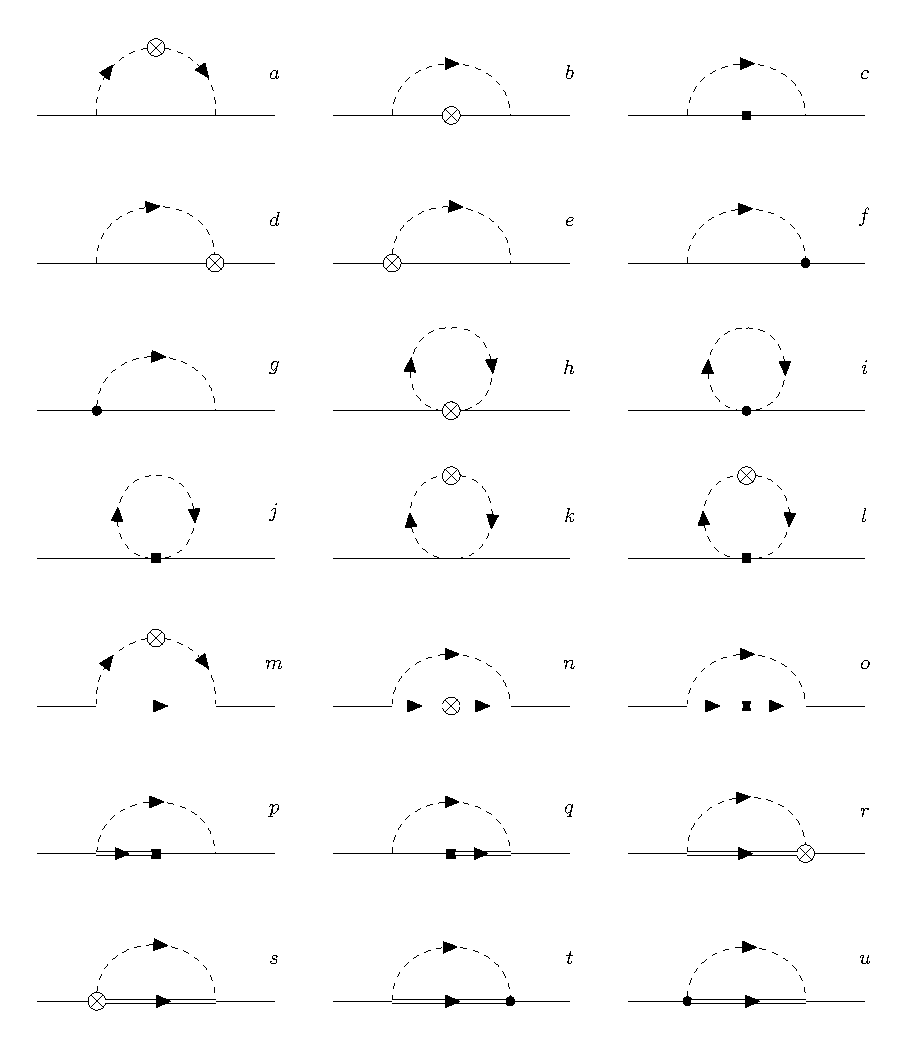
\includegraphics{23411/fig1}

\caption{the one loop Feynman diagrams}
\end{figure}

For the diagram i, the amplitude is 

\begin{align*}
\Gamma_{i}^{+} & =\bar{u}(p')\frac{C_{\phi\phi}}{f^{2}}\int\frac{d^{4}k}{(2\pi)^{4}}\tilde{F}(k)\frac{i}{D_{\phi}(k)}2\cancel{k}\frac{(2k+q)^{+}}{2kq+q^{2}}[\tilde{F}(k+q)-\tilde{F}(k)]\delta(y+\xi-\frac{k^{+}}{P^{+}})u(p)\\
 & =\bar{u}(p')[\gamma^{+}f+\frac{\sigma^{+\nu}q_{\nu}}{2M}g]u(p)
\end{align*}

To get the splitting function we need to calculate these two trace
\begin{align*}
A & =\textrm{Tr}[\Gamma_{i}^{+}(\cancel{p}+M_{N})\gamma^{+}(\cancel{p'}+M_{N})]\\
 & =\frac{C_{\phi\phi}}{f^{2}}\int\frac{d^{4}k}{(2\pi)^{4}}\textrm{Tr}[2\cancel{k}\frac{(2k+q)^{+}}{2kq+q^{2}}(\cancel{p}+M_{N})\gamma^{+}(\cancel{p'}+M_{N})]\tilde{F}(k)\frac{i}{D_{\phi}(k)}[\tilde{F}(k+q)-\tilde{F}(k)]\delta(y+\xi-\frac{k^{+}}{P^{+}})\\
 & =\int\frac{d^{4}k}{(2\pi)^{4}}(\frac{a_{1}}{D_{\phi}(k)D_{\Lambda}^{4}(k)D_{\Lambda}^{2}(k+q)}+\frac{a_{2}}{D_{\phi}(k)D_{\Lambda}^{4}(k)})\delta(y+\xi-\frac{k^{+}}{P^{+}})
\end{align*}
 
\begin{align*}
B & =\textrm{Tr}[\Gamma_{i}^{+}(\cancel{p}+M_{N})(\cancel{p'}+M_{N})]\frac{P^{+}}{M}\\
 & =\frac{C_{\phi\phi}}{f^{2}}\int\frac{d^{4}k}{(2\pi)^{4}}\textrm{Tr}[2\cancel{k}\frac{(2k+q)^{+}}{2kq+q^{2}}(\cancel{p}+M_{N})(\cancel{p'}+M_{N})]\frac{P^{+}}{M}\tilde{F}(k)\frac{i}{D_{\phi}(k)}[\tilde{F}(k+q)-\tilde{F}(k)]\delta(y+\xi-\frac{k^{+}}{P^{+}})\\
 & =\int\frac{d^{4}k}{(2\pi)^{4}}(\frac{b_{1}}{D_{\phi}(k)D_{\Lambda}^{4}(k)D_{\Lambda}^{2}(k+q)}+\frac{b_{2}}{D_{\phi}(k)D_{\Lambda}^{4}(k)})\delta(y+\xi-\frac{k^{+}}{P^{+}})
\end{align*}

where 
\[
\tilde{F}(k)=(\frac{\Lambda^{2}-m_{\phi}^{2}}{D_{\Lambda}(k)})^{2}\,D_{\Lambda}(k)=\Lambda^{2}-k^{2}
\]

If the power of the $k^{-}$ in the denominator of the integral and
the $k^{-}$ in the numerator are same when $k^{+}$ is 0 , the integral
should contain a $\delta$ term. In this case, the power of $k^{-}$
in denominator and numerator are both 2. In the previous paper, we
have some equations to calculate the $\delta$ term, one them is 
\[
\int\frac{d^{4}k}{(2\pi)^{4}}\frac{1}{D_{\phi}(k)D_{\Lambda}^{4}(k)}\delta(y+\xi-\frac{k^{+}}{P^{+}})=\int d^{2}k^{\perp}\int dx\frac{\Gamma(5)}{\Gamma(1)\Gamma(4)}\frac{1}{4!}x(1-x)^{4}\frac{\partial^{3}}{\partial^{3}\Omega}\frac{2\pi i}{k^{\perp2}+\Omega}\delta(y+\xi)
\]

So I separate the numerator of the integral in this form. First, $\textrm{numerator of }A$
can be expressed as 
\[
\textrm{numerator of }A=c_{1}(k^{-})^{2}+c_{2}k^{-}+c_{3}
\]

where $c_{i}$ represent the coefficient. Then I put the $c_{1}(k^{-})^{2}$
in this term $D_{\Lambda}^{2}(k+q)*a_{2}$ which means 
\begin{align*}
\textrm{numerator of }A & =a_{1}+D_{\Lambda}^{2}(k+q)*a_{2}\\
a_{2} & =\frac{c_{1}}{((k^{+})^{2}+2k^{+}q^{+}+(q^{+})^{2})}\\
D_{\Lambda}^{2}(k+q) & =(\Lambda^{2}-(k+q)^{2})^{2}\\
 & =((k^{+})^{2}+2k^{+}q^{+}+(q^{+})^{2})(k^{-})^{2}+...
\end{align*}

With this transition, the power of $k^{-}$ in $a_{1}$ is 1 when
$k^{+}$is 0 which means the $a_{1}$ term does not contain $\delta$
term and the $a_{2}$ is the $\delta$ term and can be calculated
using the equation.The $a_{1}$ and $a_{2}$ in diagram i is given
as
\begin{align*}
a_{1} & =2(2k^{+}+q^{+})^{2}(m_{\phi}^{2}-\Lambda^{2})^{4}\\
 & (\frac{(2k^{+}+q^{+})((k^{\perp}+q^{\perp})^{2}-k^{-}q^{+}-q^{+}q^{-}-k^{+}(k^{-}+q^{-})+\Lambda^{2})^{2}(-2P^{+}q^{+}+q^{+2}-4P^{+2}(1+\xi))}{(k^{+}+q^{+})^{2}}\\
 & +(k^{\perp2}+(k^{\perp}+q^{\perp})^{2}-2k^{+}k^{-}-k^{-}q^{+}-k^{+}q^{-}-q^{+}q^{-}+2\Lambda^{2})\\
 & *(2(k^{\perp}+q^{\perp})^{2}P^{+}-4(p^{\perp}-k^{\perp})^{2}P^{+}-4M_{N}^{2}P^{+}-4k^{-}P^{+2}\\
 & -4k^{+}P^{+}P^{-}+4P^{+2}P^{-}-(k^{\perp}+q^{\perp})^{2}q^{+}-2k^{-}P^{+}q^{+}+k^{-}q^{+2}\\
 & +k^{\perp2}(2P^{+}+q^{+})-2k^{+}P^{+}q^{-}+k^{+}q^{+}q^{-}-2P^{+}q^{+}q^{-}+q^{+2}q^{-}\\
 & -4k^{-}P^{+2}\xi+4P^{+2}P^{-}\xi-(2k^{+}-2P^{+}+q^{+})q^{2})\\
a_{2} & =\frac{2(2k^{+}+q^{+})^{2}(m_{\phi}^{2}-\Lambda^{2})^{4}}{(k^{+}+q^{+})^{2}}(2P^{+}q^{+}-q^{+2}+4P^{+2}(1+\xi))
\end{align*}
 

Then we can get the normal and $\delta$ term of $f$ and $g$

\begin{align*}
f & =f_{res}+\delta f\\
g & =g_{res}+\delta g
\end{align*}

The $g$ is 0 for diagram i. The $f_{res}$ is showed in fig.2. And
the $\delta$ term, $\delta f=-0.0977421\delta(y+\xi)$. The result
of $f$ and $g$ can be checked by compare the integral with the previous
form factor work.
\begin{equation}
F_{1}=\widetilde{F}(q)\int dy(f_{res}+\delta f)
\end{equation}

where $\widetilde{F}(q)$ is the regulator of photon which we introduce
by hand in form factor calculation to get the $Q^{2}$ dependence.
In GPD calculation this $Q$ dependence comes from the input GPD.
The result of eq.1,with $Q^{2}=1$ is $0.0324215\widetilde{F}(1)=0.00810537$,
while the result in form factor is $0.00810465$

\begin{figure}
\includegraphics[scale=0.5]{424/fres-xi0\lyxdot 1}

\caption{$f_{res}$($\xi=0.1,Q^{2}=1GeV^{2}$) }

\end{figure}

The positive part of $f_{res}$ is small but not zero which is showed
in Fig.3. To check whether the $f_{res}$ is $\delta$ function when
$\xi$ is 0, I have these $\xi f_{res}$ figure showed in Fig.4.

\begin{figure}
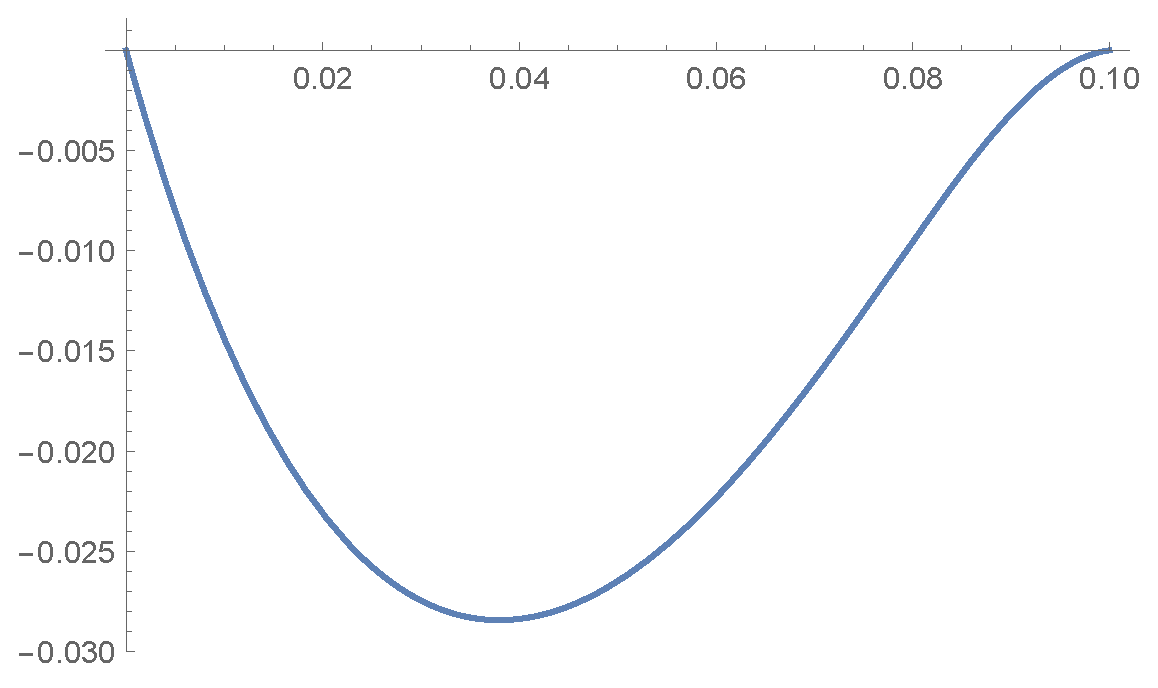
\includegraphics[scale=0.5]{424/fres-zheng}\caption{$f_{res}(y),y>0$}

\end{figure}

\begin{figure}
\includegraphics[scale=0.5]{424/xi-fres-delta}

\caption{$\xi f_{res}$ with $\xi=0.1,0.01,0.001,0.0001$}
\end{figure}

Still the positive part is not zero and is showed in Fig.5. And these
two figure prove that $f_{res}$ approach to the $\delta(y)$ in the
zero skewness limit despite in different method. 

\begin{figure}
\includegraphics[scale=0.5]{424/xi-fres-zheng}

\caption{$\xi f_{res}(y),y>0$ }

\end{figure}

For diagram b in Fig1, the contribution is 
\[
\Gamma_{b}^{+}=\int\cancel{k}\gamma_{5}\widetilde{F}^{2}(k)\frac{1}{D_{\phi}(k)}\frac{\cancel{p'}-\cancel{k}+m_{N}}{D_{B}(p'-k)}\gamma^{+}\frac{\cancel{p}-\cancel{k}+m_{N}}{D_{B}(p-k)}\cancel{k}\gamma_{5}\delta(y+\xi-\frac{k^{+}}{P^{+}})
\]

I do the same separate in diagram i case. The $A$ part is 
\begin{align*}
A_{b} & =\text{\ensuremath{\int(\Lambda^{2}-m_{\phi}^{2})^{4}\frac{\textrm{Tr}[\cancel{k}\gamma_{5}(\cancel{p'}-\cancel{k}+m_{N})\gamma^{+}(\cancel{p}-\cancel{k}+m_{N})\cancel{k}\gamma_{5}]}{D_{\Lambda}^{4}(k)D_{\phi}(k)D_{B}(p'-k)D_{B}(p-k)}}}\delta(y+\xi-\frac{k^{+}}{P^{+}})\\
 & =\int\frac{d^{4}k}{(2\pi)^{4}}(\frac{b_{1}}{D_{\Lambda}^{4}(k)D_{\phi}(k)D_{B}(p'-k)D_{B}(p-k)}+\frac{b_{2}}{D_{\phi}(k)D_{\Lambda}^{4}(k)})\delta(y+\xi-\frac{k^{+}}{P^{+}})
\end{align*}

Then first term is normal integral which can be calculated with residue
theorem and the second term is $\delta$ term. The normal part can
be expressed as 
\begin{multline*}
\int\frac{d^{4}k}{(2\pi)^{4}}\frac{b_{1}}{D_{\Lambda}^{4}(k)D_{\phi}(k)D_{B}(p'-k)D_{B}(p-k)}\delta(y+\xi-\frac{k^{+}}{P^{+}})\\
=\int\frac{d^{4}k}{(2\pi)^{4}}(\frac{b'_{1}k^{-}}{D_{\Lambda}^{4}(k)D_{\phi}(k)D_{B}(p'-k)D_{B}(p-k)}+\frac{b_{1}''}{D_{\Lambda}^{4}(k)D_{\phi}(k)D_{B}(p'-k)D_{B}(p-k)})\delta(y+\xi-\frac{k^{+}}{P^{+}})
\end{multline*}

This week, I check the integral above. The integral should have no
issue and the contribution of diagram b can be calculated using the
similar method as diagram i. Last week I made a mistake in my program.
The splitting function can be expressed as
\begin{align*}
f & =f_{1}+f_{2}+f_{\delta}\delta(y+\xi)\\
g & =g_{1}+g_{2}+g_{\delta}\delta(y+\xi)
\end{align*}

the $f_{1}+f_{2}$ means the normal part of the splitting function
which is separated in $k^{+}=(1-\xi)P^{+}$ due to the singularity
comes from $D_{B}(p'-k)=(p'-k)^{2}-M^{2}+i\epsilon$ change it's position
from upside to the down side of the axis and the $f_{\delta}\delta(y+\xi)$
is the $\delta$ term. 

The splitting function should satisfy that $\int_{-\xi}^{1}dyf(y)$
and $\int_{-\xi}^{1}dyg(y)$ are $\xi$ independent. For diagram b,
the result is, with $\xi=0.1,0.2$, ignore some coefficient
\[
\int_{-\xi}^{1-2\xi}dyf_{1}(y)+\int_{1-2\xi}^{1}dyf_{2}(y)+f_{\delta}=7.27795
\]

and 
\[
\int_{-\xi}^{1-2\xi}dyg_{1}(y)+\int_{1-2\xi}^{1}dyg_{2}(y)+g_{\delta}=-6.566548599
\]

When $\xi=0.1,Q^{2}=1GeV^{2}$, the splitting function looks like
this 
\begin{figure}
\includegraphics{pic/b-f1}

\caption{$f_{1}$from diagram b}

\end{figure}

\begin{figure}
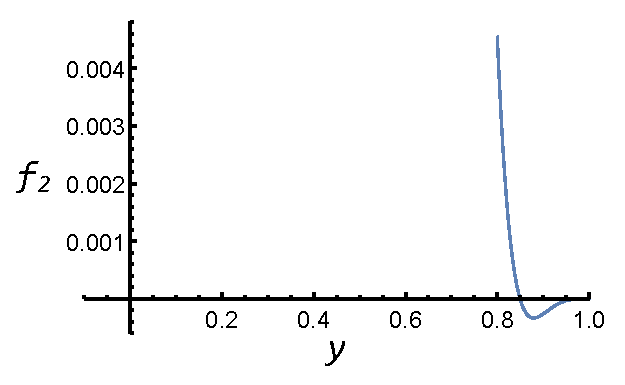
\includegraphics{pic/b-f2}

\caption{$f_{2}$from diagram b}

\end{figure}

\begin{figure}
\includegraphics{pic/b-g1}

\caption{$g_{1}$from diagram b}
\end{figure}

\begin{figure}
\includegraphics{pic/b-g2}

\caption{$g_{2}$from diagram b}
\end{figure}

The $\delta$ term is 
\begin{align*}
f_{\delta}\delta(y+\xi) & =5.2702\delta(y+\xi)\\
g_{\delta}\delta(y+\xi) & =0
\end{align*}

Second, I don't think we need to consider the point contribution in
Chueng-Ryong's paper. The two integral below
\begin{align*}
\int dk^{-}\frac{k^{-}}{D_{\Lambda}^{4}(k)D_{\phi}(k)D_{B}(p'-k)D_{B}(p-k)}\\
\int dk^{-}\frac{1}{D_{\Lambda}^{4}(k)D_{\phi}(k)D_{B}(p'-k)D_{B}(p-k)}
\end{align*}

are not corresponding to this integral in the paper 
\[
V=\int d^{2}k\frac{k^{-}}{(k^{2}-m_{1}^{2})((k-p)^{2}-m_{2}^{2})}
\]

Because the above two integrals converge when $k^{+}=0$. In the asymptotic
method part of the paper, the $V$ is separated to three part,
\begin{align*}
V & =\frac{1}{2}\int dk^{+}dk^{-}\frac{-p^{-}k^{+}+p^{2}+m_{1}^{2}-m_{2}^{2}}{(k^{2}-m_{1}^{2})((k-p)^{2}-m_{2}^{2})}\\
 & -\frac{1}{2p^{2}}\int dk^{+}dk^{-}\frac{p^{-}}{(k^{2}-m_{1}^{2})}+\frac{1}{2p^{2}}\int dk^{+}dk^{-}\frac{p^{-}}{((k-p)^{2}-m_{2}^{2})}
\end{align*}
 The first term is converged and can bu calculated with residue theorem.
The second and third term are divergences. This is similar to the
separation of $\delta$ term and normal term. So the normal term should
not consider the extra contribution from $k^{+}=0$ which should be
contained in the $\delta$ term.
\end{document}
